
\chapter{Resultados}

\section{Análisis de Límites Teóricos (Oracle Upper Bounds)}

Para evaluar el potencial máximo de la estrategia de adaptación híbrida y establecer un techo teórico de desempeño, se diseñaron dos experimentos de búsqueda exhaustiva.

La metodología consiste en procesar la nube de puntos completa, bloque por bloque, evaluando todas las combinaciones posibles de los parámetros de adaptación en un espacio de búsqueda granular:

\begin{itemize}
    \item \textbf{Espacio de búsqueda:} Se evaluaron porcentajes de selección de nodos $p \in [0.01, 1.00]$ con incrementos de $0.02$, y pesos de auto-lazo $w \in [0.2, 10.2]$ con incrementos de $0.2$.
    \item \textbf{Absolute Oracle:} Utiliza la señal de luminancia original (ground truth) para calcular el vector de importancia de los nodos y guiar la inserción de auto-lazos. Representa el límite superior si el sistema tuviera conocimiento perfecto de la señal antes de la transformada.
    \item \textbf{Linear Oracle:} Utiliza una aproximación lineal (ajuste de plano por mínimos cuadrados) de la luminancia. Este experimento busca determinar si una representación simplificada y robusta de la señal conserva la efectividad del método con datos reales.
\end{itemize}

Para cada bloque y cada paso de cuantización ($Q=\{24, 32, 48, 64\}$), el decisor RDO selecciona la combinación $(p, w)$ que minimiza el costo $J = R + \lambda D$. Los resultados agregados permiten cuantificar la eficiencia máxima alcanzable mediante métricas Bjontegaard.

\subsection{Métricas Bjontegaard y Eficiencia RD}


La Tabla \ref{tab:oracle_comparison} presenta las métricas BD-Rate y BD-PSNR de ambos oráculos comparadas con el método básico estructural. 

\begin{table}[ht]
\centering
\caption{Comparativa de Métricas Bjontegaard: Absolute Oracle vs. Linear Oracle}
\begin{tabular}{|c|c|c|c|}
\hline
\textbf{Tamaño de Bloque} & \textbf{Métrica} & \textbf{Absolute Oracle} & \textbf{Linear Oracle} \\
\hline
\multirow{2}{*}{4} & BD-Rate (\%) & -16.00\% & -19.20\% \\
                   & BD-PSNR (dB) & 1.44 & 1.80 \\
\hline
\multirow{2}{*}{8} & BD-Rate (\%) & -17.69\% & -23.57\% \\
                   & BD-PSNR (dB) & 0.95 & 1.31 \\
\hline
\multirow{2}{*}{16} & BD-Rate (\%) & -9.22\% & -14.71\% \\
                    & BD-PSNR (dB) & 0.42 & 0.68 \\
\hline
\end{tabular}
\label{tab:oracle_comparison}
\end{table}

\subsection{Interpretación de Resultados}

Un hallazgo fundamental de estos experimentos es que el \textbf{Linear Oracle supera consistentemente al Absolute Oracle}, logrando entre un 120\% y un 160\% de la reducción de tasa de bits esperada. Este fenómeno puede explicarse mediante la teoría tasa-distorsión y las métricas de Bjoontgard:

\begin{itemize}
    \item \textbf{Efecto de Filtro Paso Bajo:} El Linear Oracle utiliza una superficie plana ajustada, lo que actúa como un filtro paso bajo espacial. Al ignorar el ruido de alta frecuencia y las variaciones locales, la adaptación del grafo se guía por la tendencia global del bloque, lo que resulta en una base GFT más eficiente para compactar la energía de la señal.
    \item \textbf{Compacidad de Energía:} Las funciones de base derivadas de la aproximación lineal se alinean mejor con los componentes de baja frecuencia, que contienen la mayor parte de la información visual.
    \item \textbf{Sensibilidad al Tamaño del Bloque:} Las mayores ganancias se observan en bloques de $8 \times 8$. Para bloques de $16 \times 16$, aunque el Linear Oracle sigue siendo superior, la precisión de la aproximación lineal disminuye para superficies complejas.
\end{itemize}

\begin{figure}[ht]
    \centering
    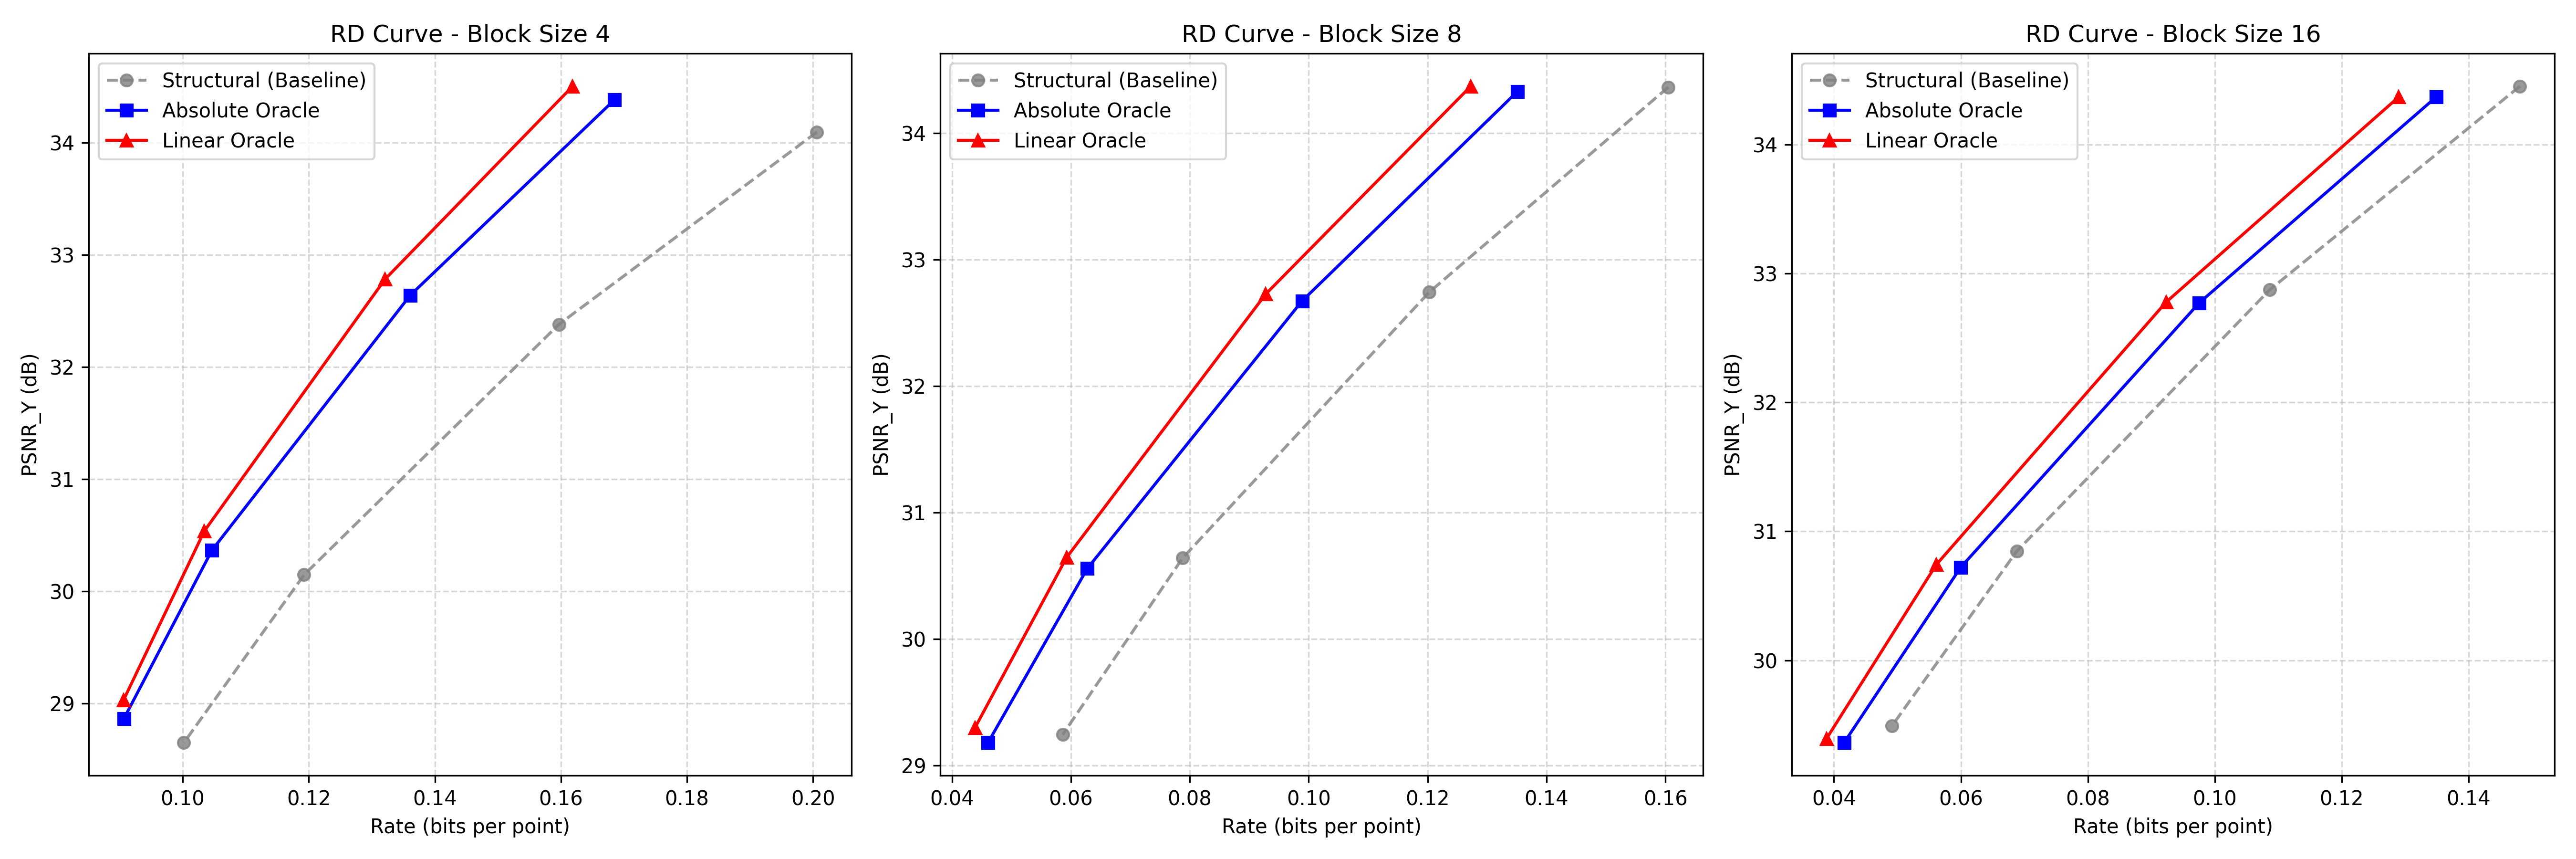
\includegraphics[width=1.0\linewidth]{img/resultados/rd_curves_comparison.png}
    \caption{Curvas Rate-Distortion para diferentes tamaños de bloque comparando la línea base con ambos oráculos.}
    \label{fig:rd_curves_oracle}
\end{figure}

\begin{figure}[ht]
    \centering
    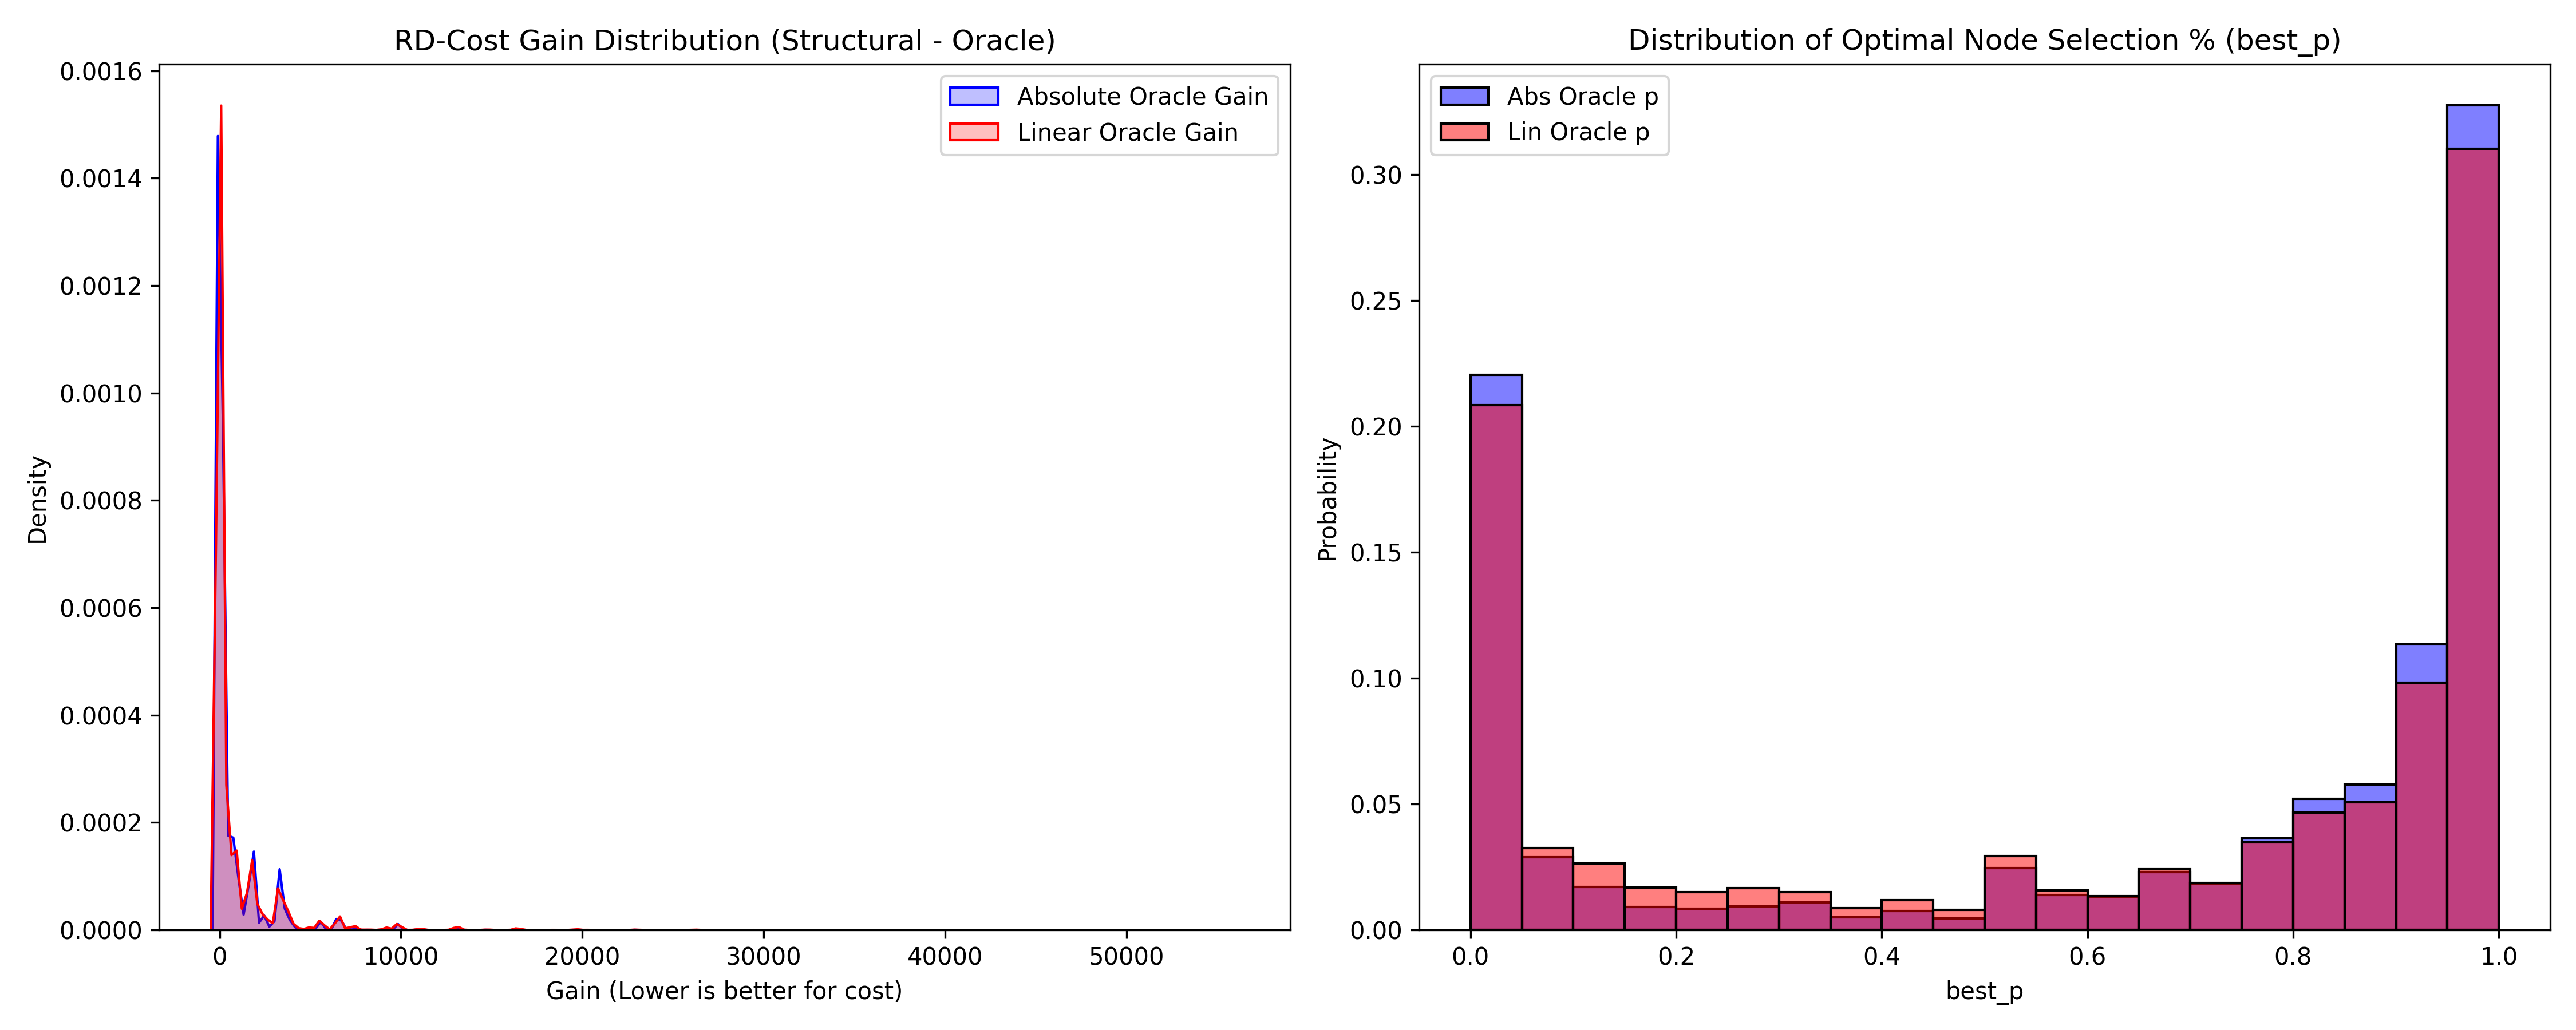
\includegraphics[width=0.8\linewidth]{img/resultados/gain_parameters_analysis.png}
    \caption{Análisis de distribución de ganancias y parámetros óptimos de selección de nodos ($p$).}
    \label{fig:gain_analysis}
\end{figure}

Como se observa en la Figura \ref{fig:gain_analysis}, la distribución de los parámetros óptimos se mantiene estable para ambas ejecuciones del oráculo. Esta consistencia es fundamental, ya que sugiere que el comportamiento del sistema no es errático ante diferentes aproximaciones de la señal. Por consiguiente, es viable realizar un paso posterior de agrupación (clustering) de estos parámetros, lo que permitiría una representación compacta de la configuración de adaptación con un overhead de señalización mínimo en el flujo de bits final.

\section{Análisis de Sensibilidad y Agrupamiento RD (RD-Clustering)}

En esta sección se presentan los resultados de la estrategia de agrupamiento conjunta de pendientes y parámetros de auto-lazo ($S_x, S_y, S_z, SLW, SLP$). El objetivo es evaluar la estabilidad del sistema, su capacidad de aprendizaje y los límites de saturación del libro de códigos.

\subsection{Saturación de Capacidad y Resolución Estructural}

Se evaluó el comportamiento del costo RD final en función del número de clusters ($C$) para diferentes tamaños de bloque.

\begin{figure}[ht]
    \centering
    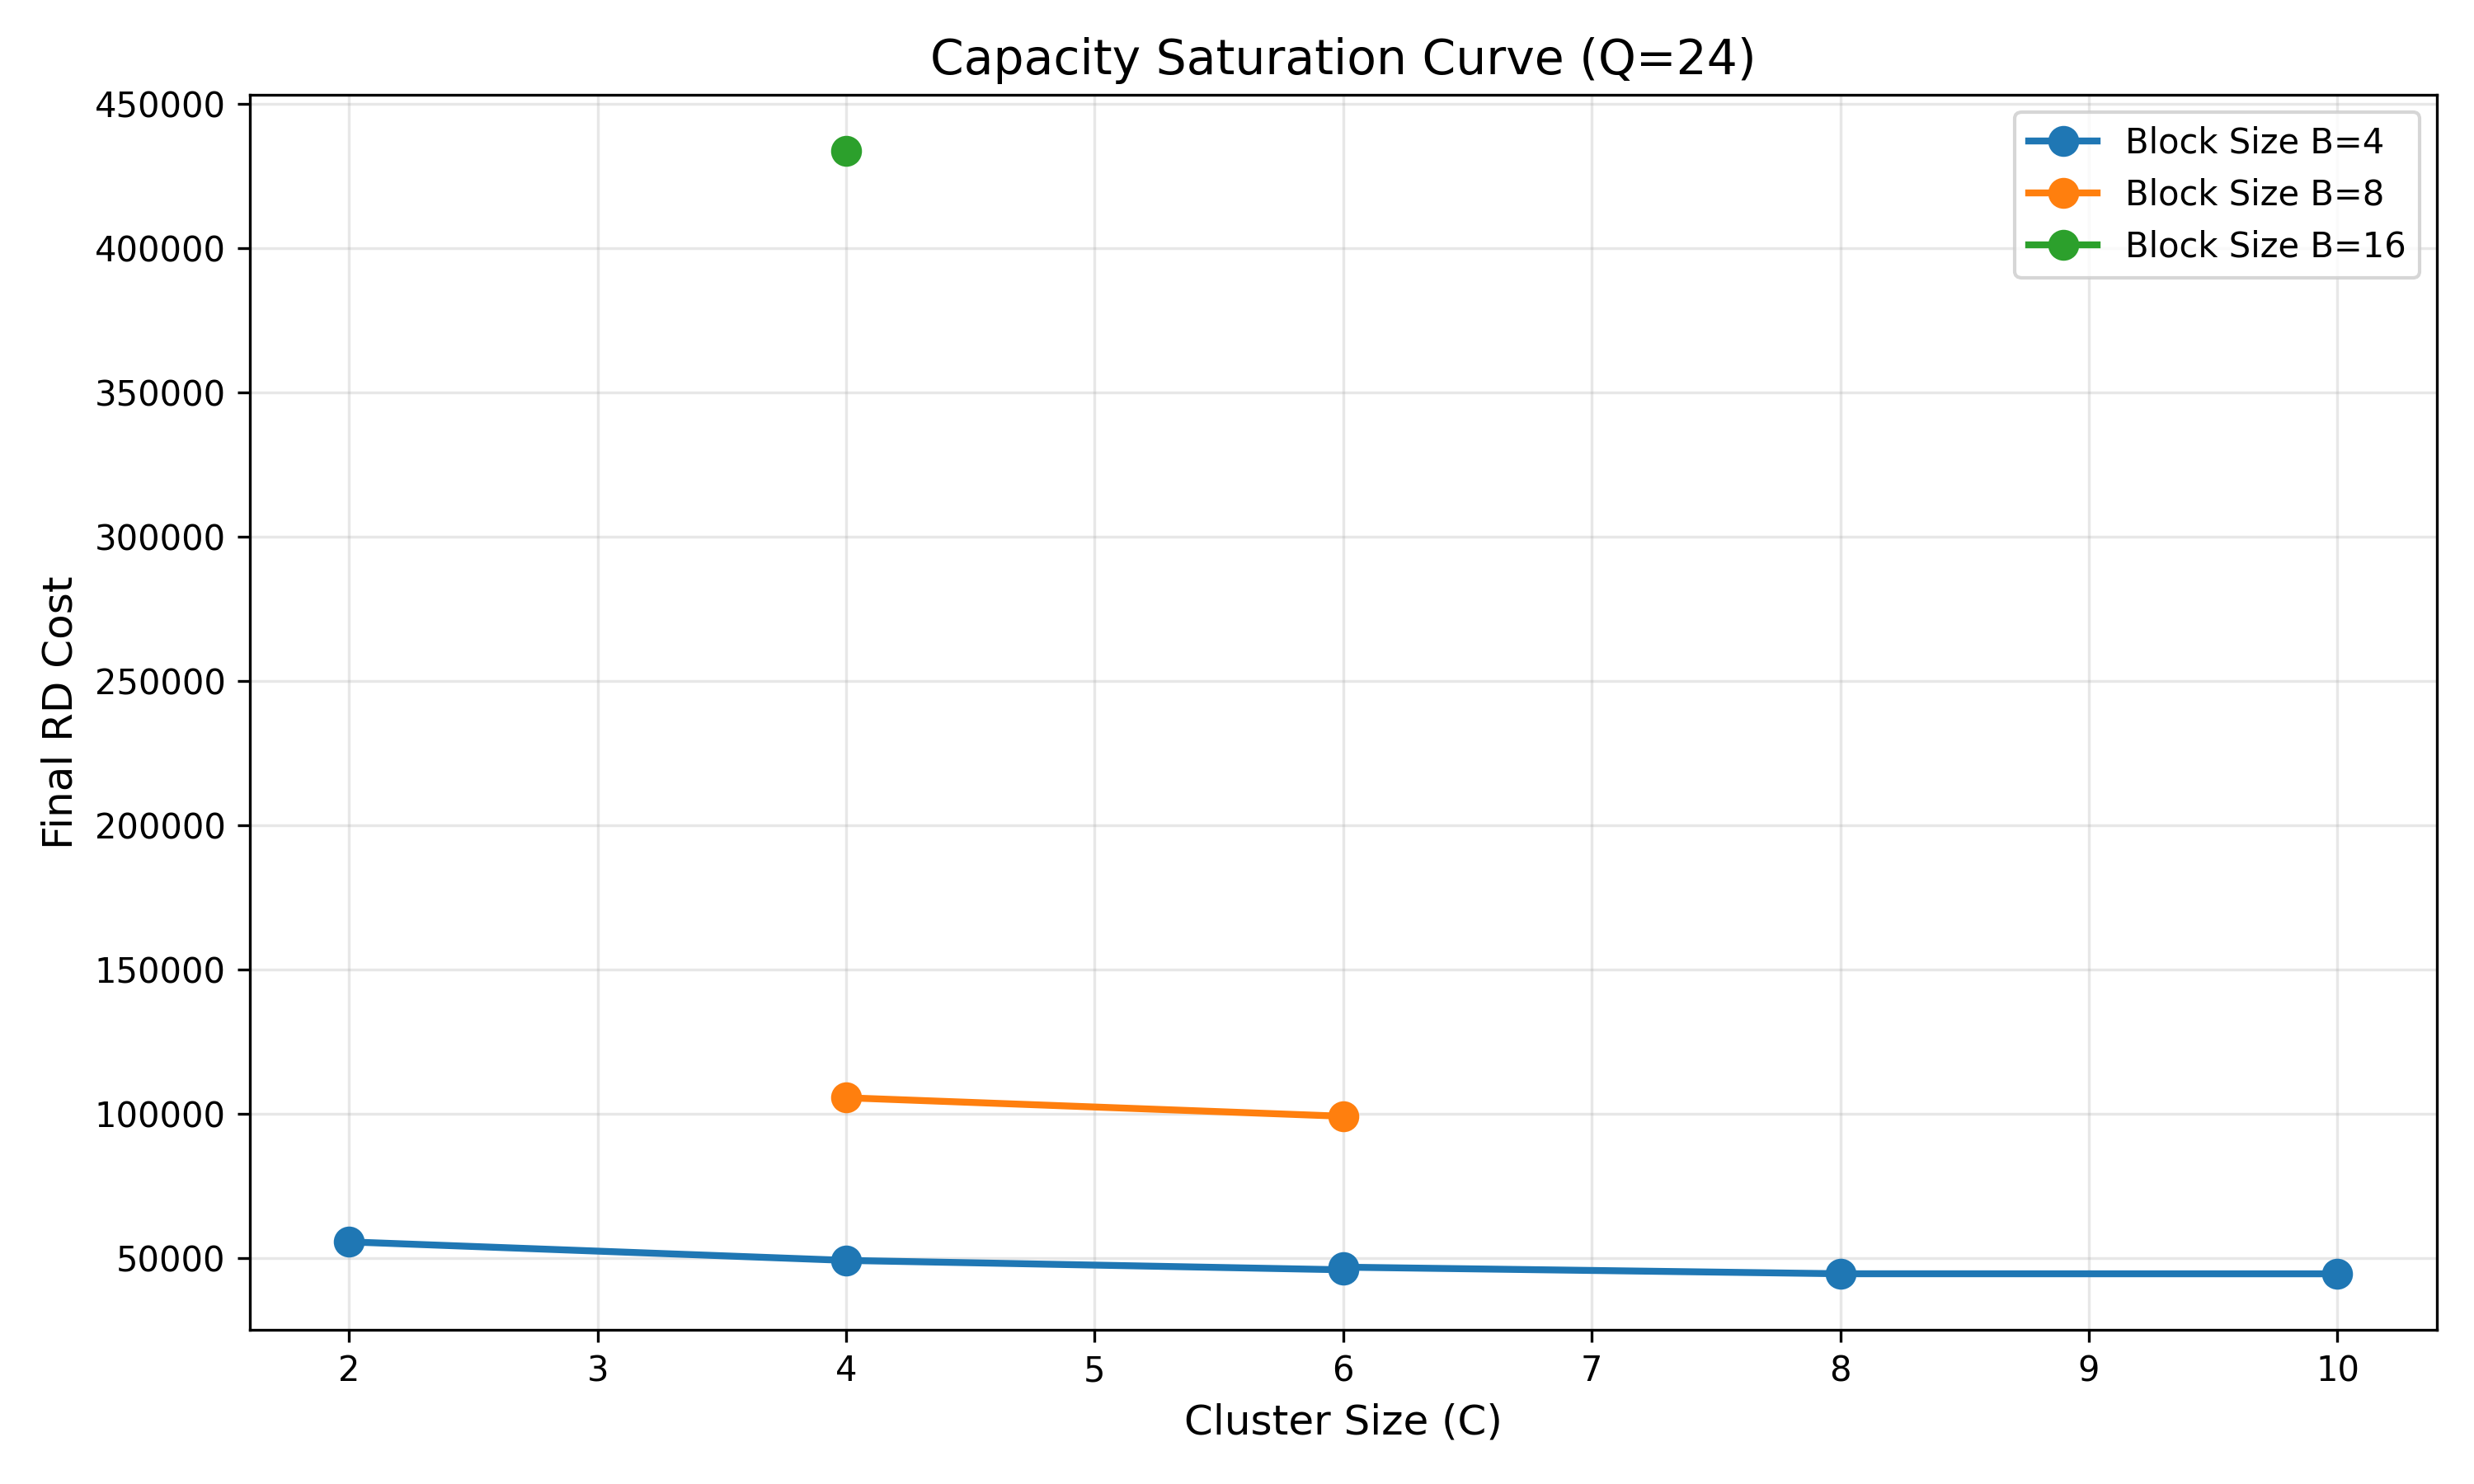
\includegraphics[width=0.8\linewidth]{img/resultados/capacity_saturation.png}
    \caption{Curva de saturación de capacidad para diferentes tamaños de bloque (Q=24).}
    \label{fig:capacity_saturation}
\end{figure}

% --- ESPACIO PARA ESCRITURA ---
% Sugerencia: Analizar cómo B=4 responde mejor al incremento de C y dónde se observa el plateau.


\subsection{Trayectoria de Aprendizaje y Sparsification del Grafo}

La evolución de los parámetros de auto-lazo durante el proceso iterativo revela la estrategia de optimización del sistema para reducir la tasa de bits.

\begin{figure}[ht]
    \centering
    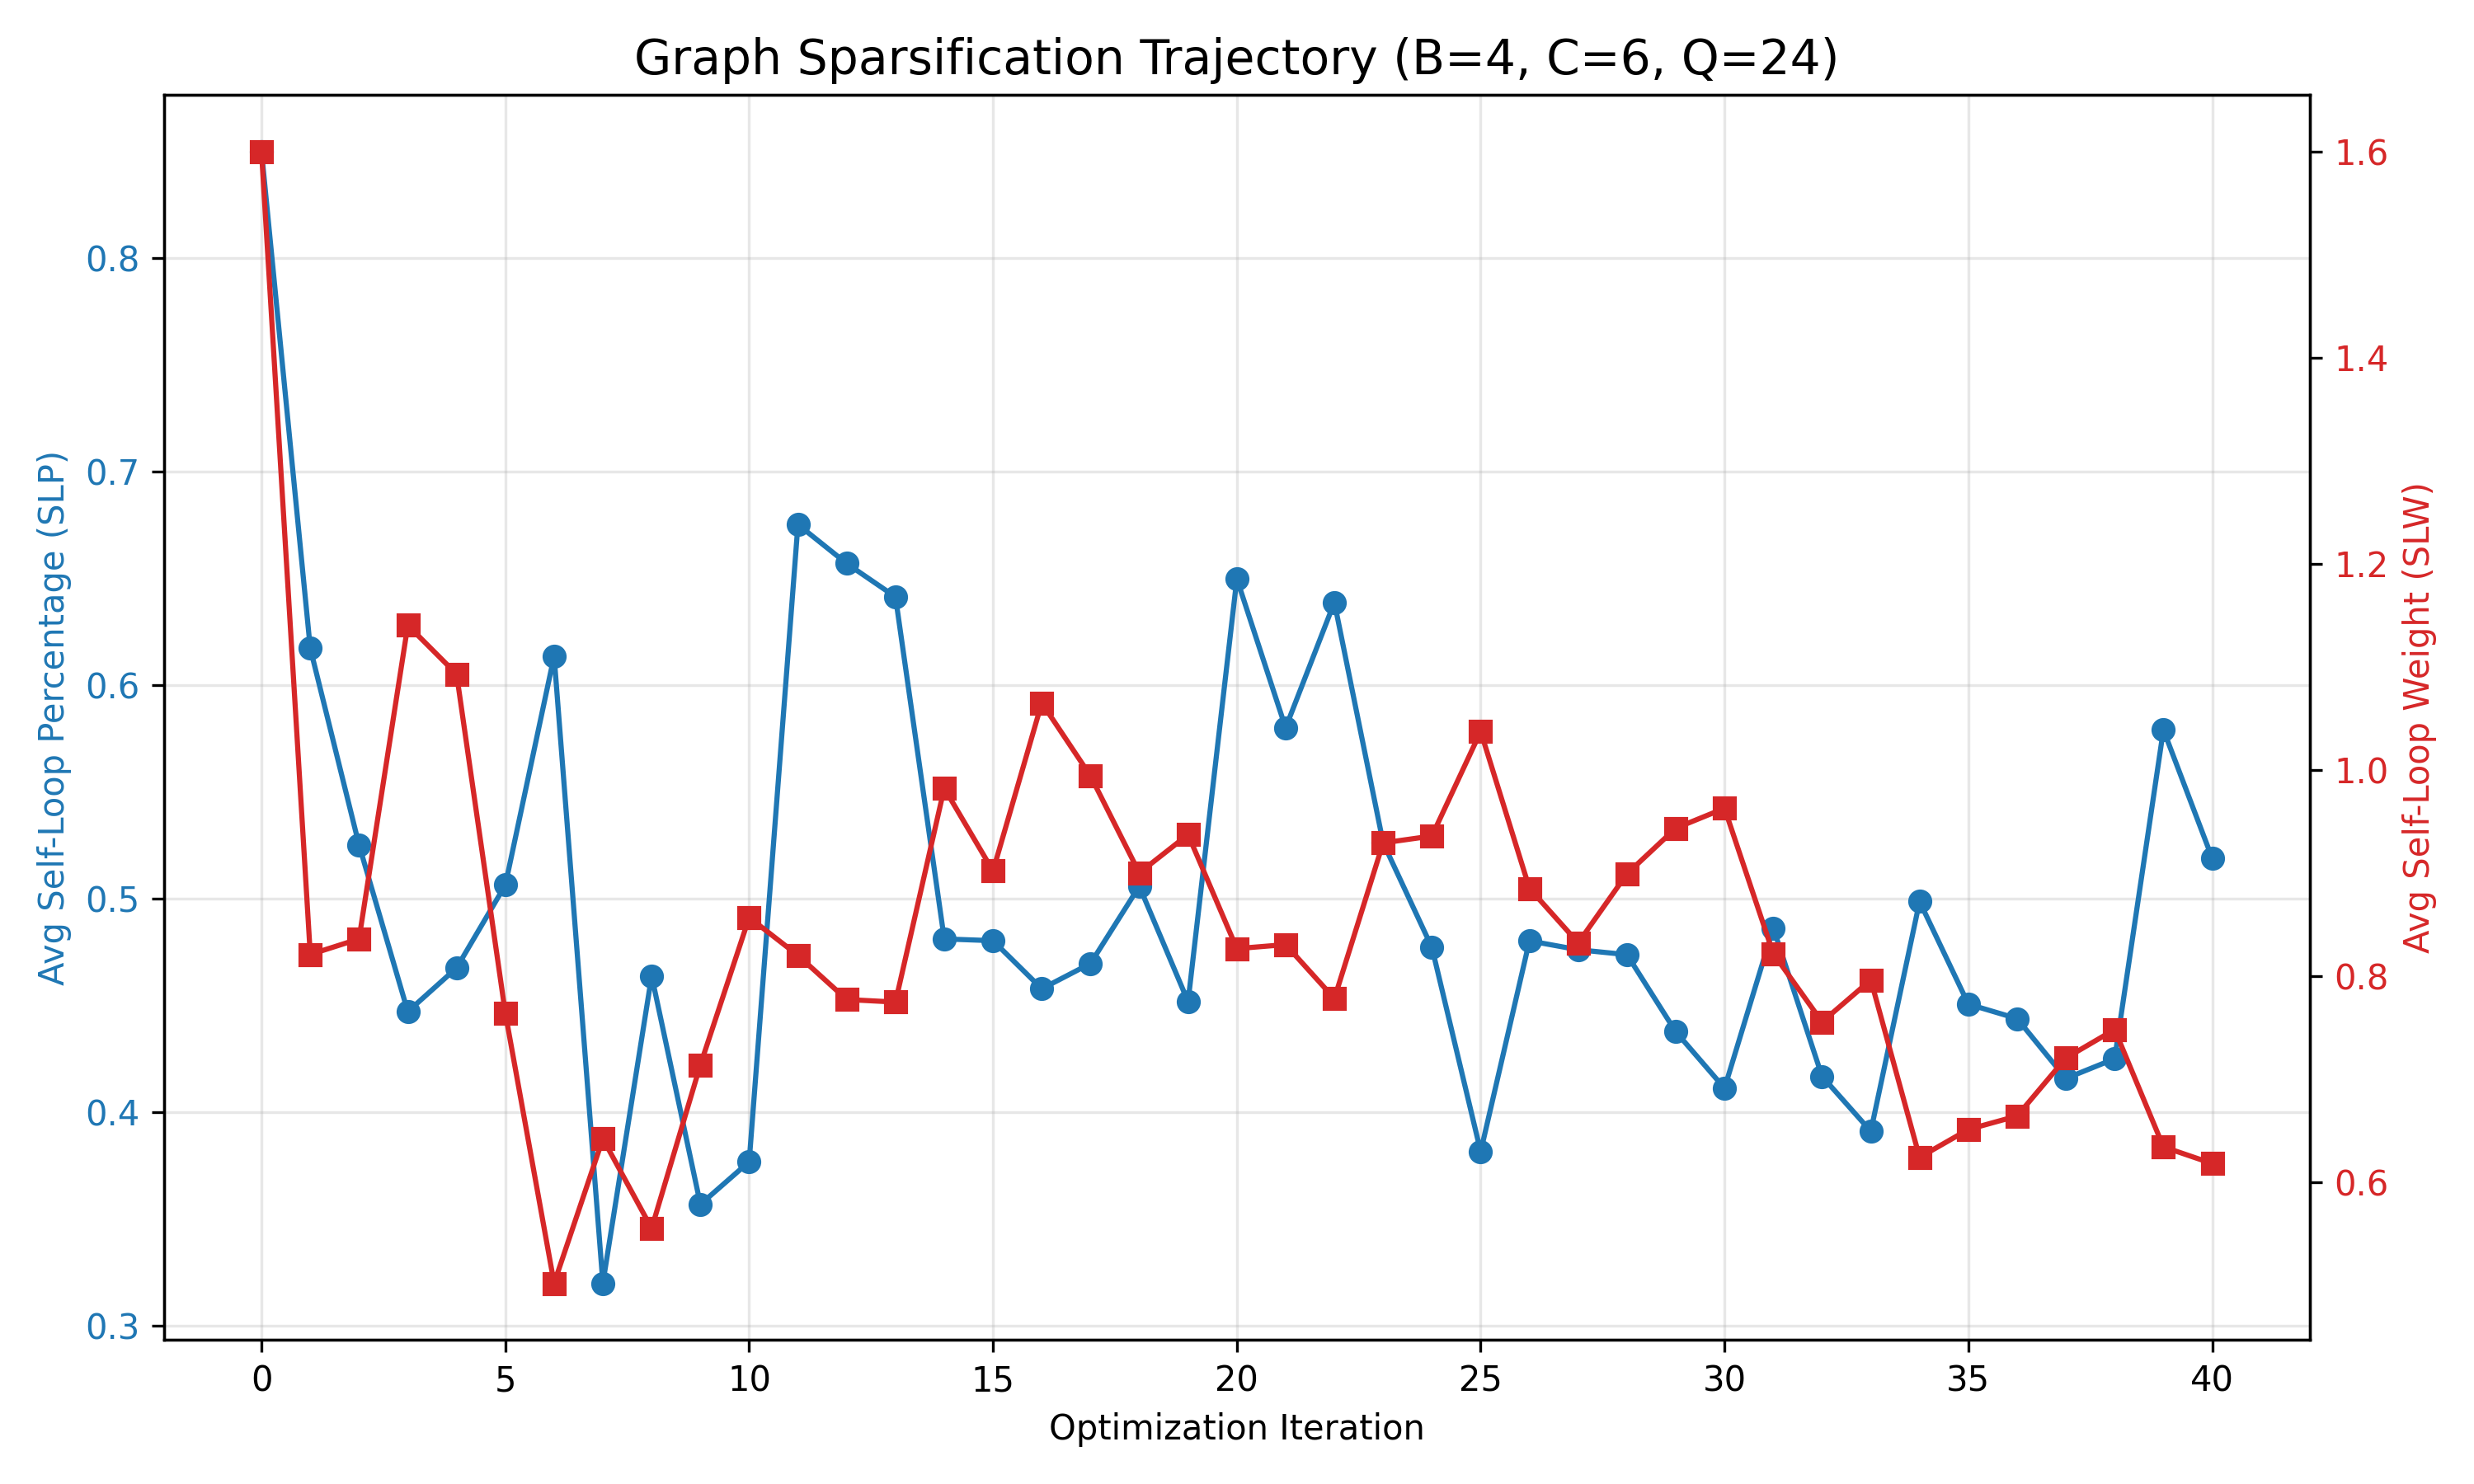
\includegraphics[width=0.8\linewidth]{img/resultados/parameter_drifts.png}
    \caption{Evolución temporal de los parámetros SLP y SLW (B=4, C=6, Q=24).}
    \label{fig:parameter_drifts}
\end{figure}

% --- ESPACIO PARA ESCRITURA ---
% Sugerencia: Comentar la caída drástica de SLP y qué significa para la conectividad del grafo.


\subsection{Velocidad de Convergencia e Impacto de la Inicialización}

Se analiza el esfuerzo de reasignación (distancia Hamming) y la velocidad con la que el sistema alcanza un estado estable.

\begin{figure}[ht]
    \centering
    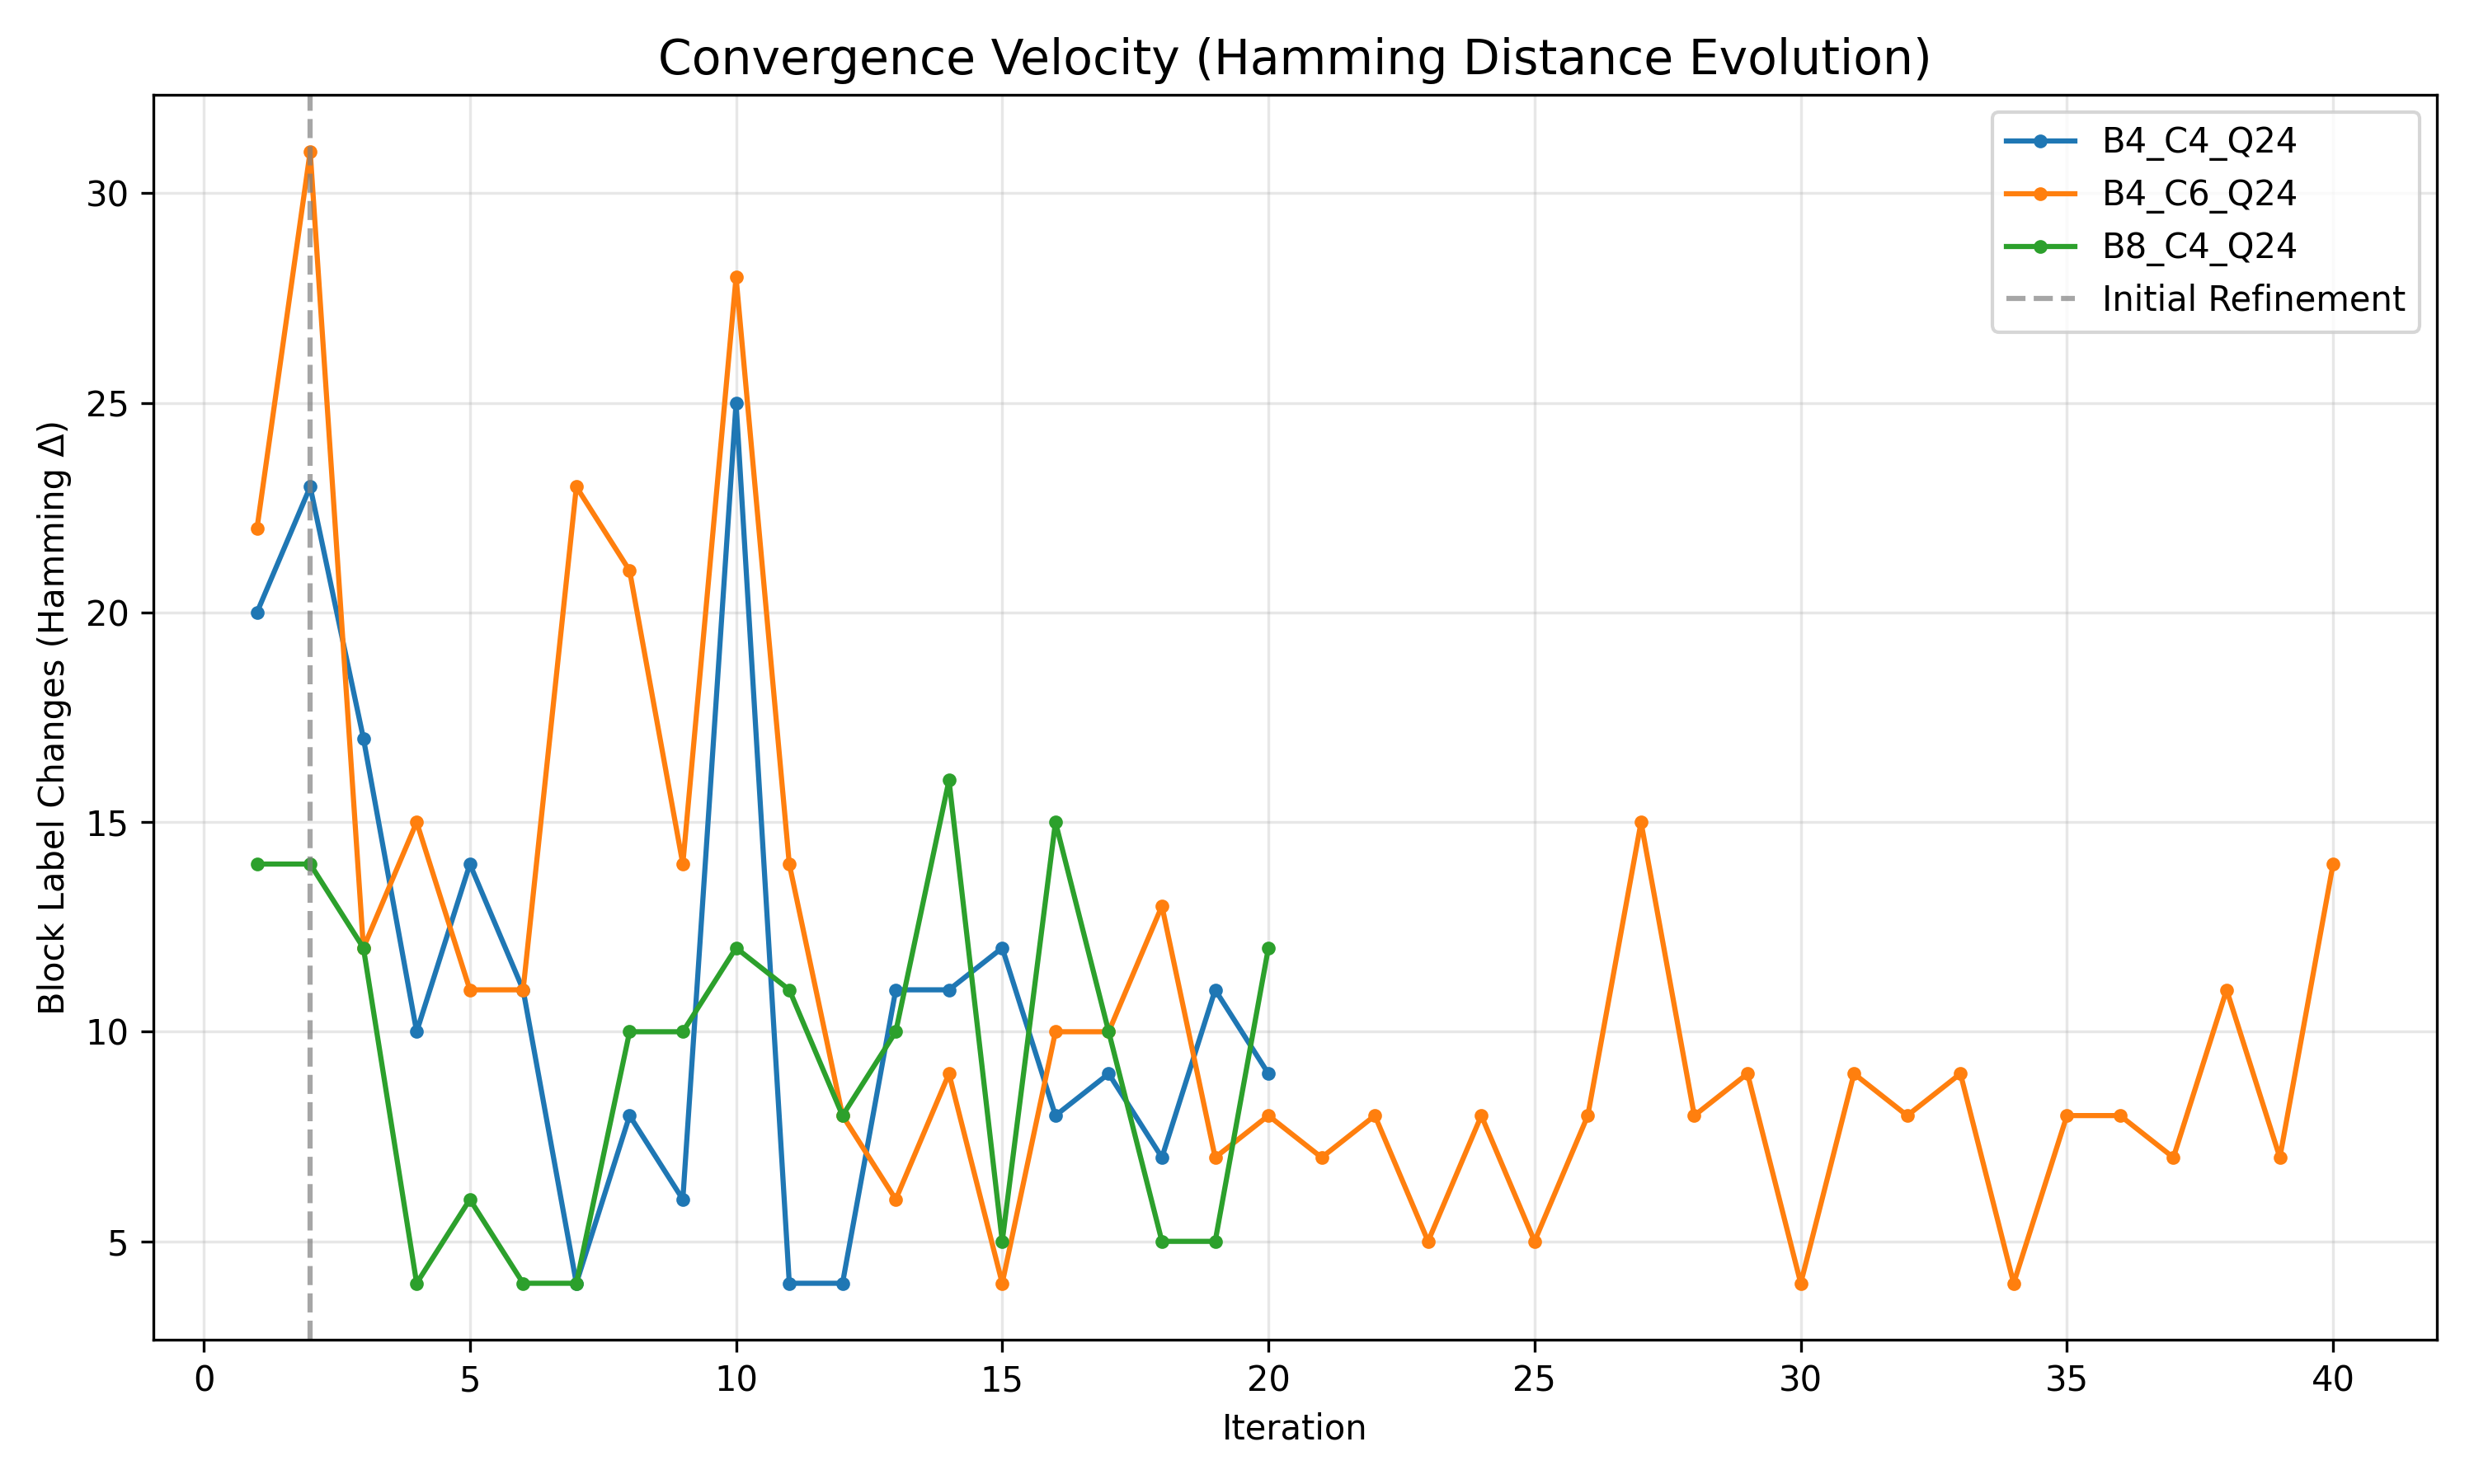
\includegraphics[width=0.8\linewidth]{img/resultados/convergence_velocity.png}
    \caption{Evolución de la distancia Hamming (reasignaciones de bloques) por iteración.}
    \label{fig:convergence_velocity}
\end{figure}

% --- ESPACIO PARA ESCRITURA ---
% Sugerencia: Describir el "Iter 2 Breakthrough" y la persistencia de cambios en configuraciones complejas.


\subsection{Frontera de Eficiencia Informacional}

Finalmente, se mapea la relación entre la ganancia obtenida y el costo de señalización (entropía) requerido para transmitir los índices de los clusters.

\begin{figure}[ht]
    \centering
    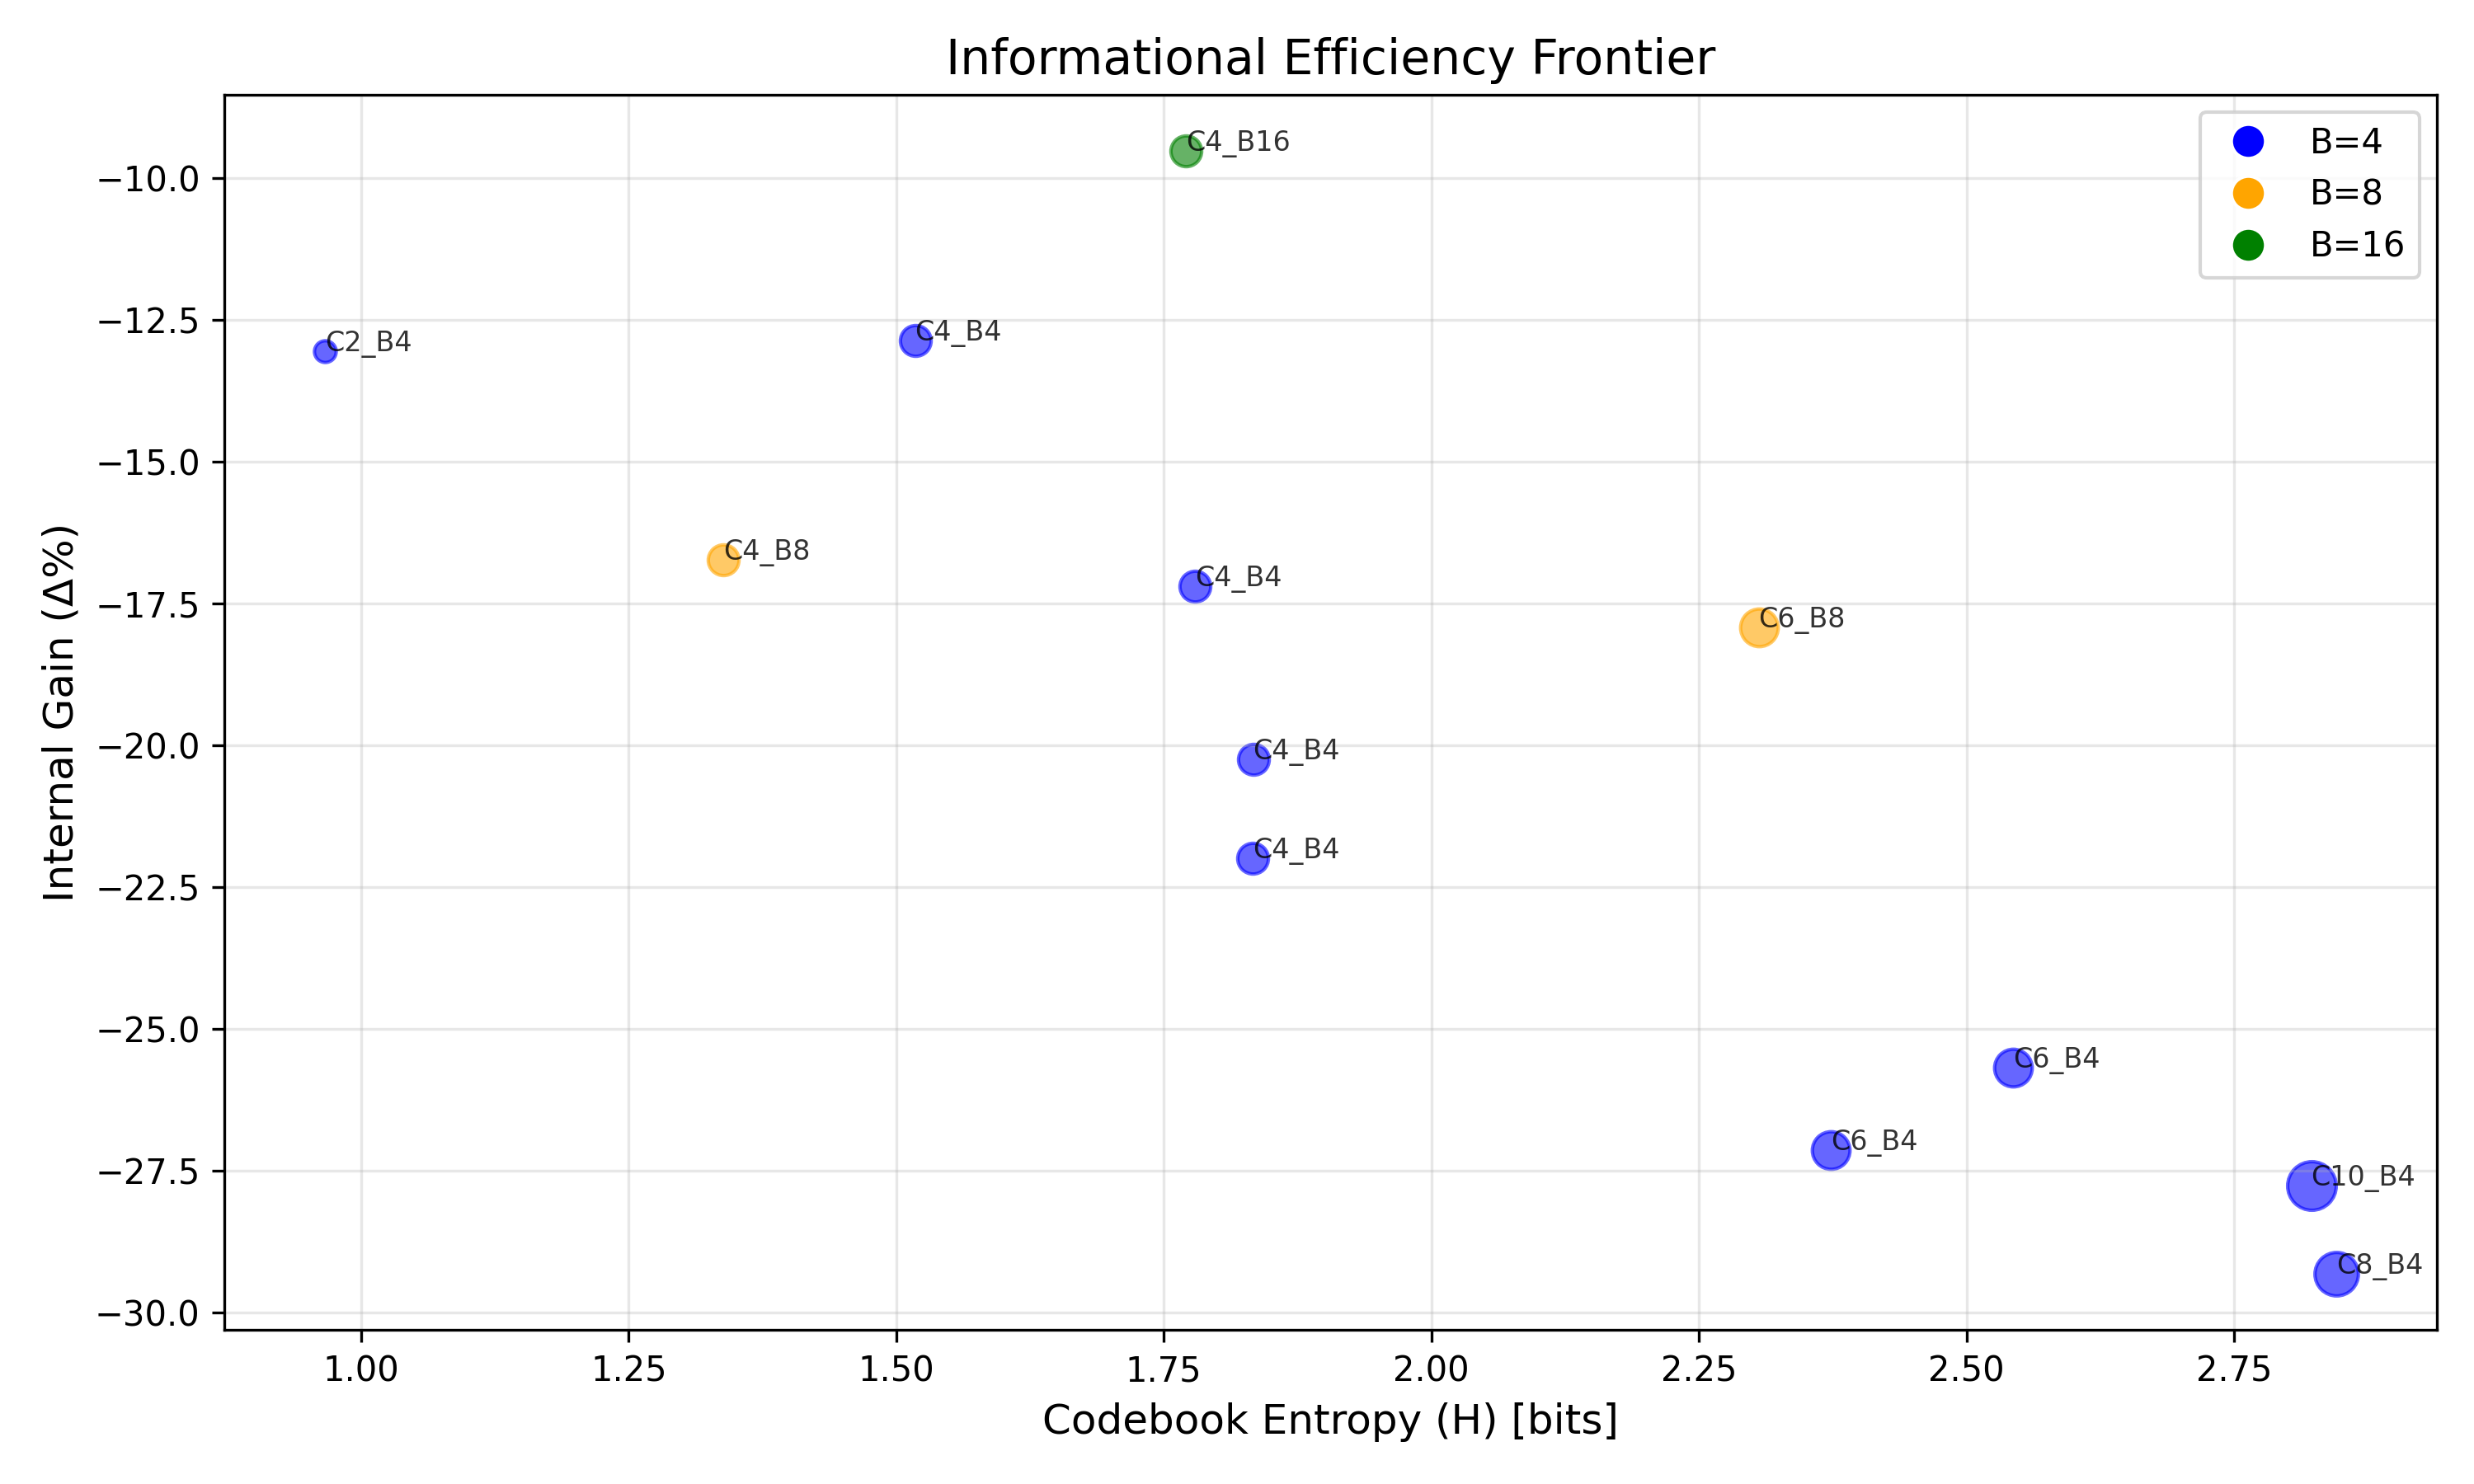
\includegraphics[width=0.8\linewidth]{img/resultados/efficiency_frontier.png}
    \caption{Frontera de Pareto: Entropía del libro de códigos vs. Ganancia Interna.}
    \label{fig:efficiency_frontier}
\end{figure}

% --- ESPACIO PARA ESCRITURA ---
% Sugerencia: Discutir qué configuraciones (C, B) ofrecen la mejor relación ganancia/overhead.

